\newpage
\chapter{Jet reconstruction and Tagging in ATLAS}
\label{Jet}
Jet object and specifically $b$-quark jet are also crucial to study the \HHyybb properties. Jets in ATLAS are currently reconstructed in two ways (EMTopo and PFlow) as explained in Section \ref{chap2:Objects:Jet}. This chapter details jet reconstruction, $b$-jet identification and calibration. I implemented a calibration method specific to $b$-jets which provides better reconstruction performances, thus better $m_{\bar{b}b}$ invariant mass resolution compared to generic jet corrections which are driven by light jets.

\section{Reconstruction algorithm}
\label{Jet:JR}
For both jet types at Run-2, jet reconstruction starts with a clustering algorithm based on calorimeter objects to form the topological cluster \cite{Jet_Algo_Perf}. The algorithm identifies calorimeter cells with energy larger than 4 $\sigma_{noise}$ (expected noise standard deviation) as cluster seeds. Then, neighbouring cells with $|E_{cell}| > 2\sigma_{noise}$ are grouped to form the cluster as well as all adjacent cells. Clusters with two or more local energy maxima are split in two with cells being associated with each maximum according to their relative distance. \\
The EMTopo jets are built later by using the Anti-$k_t$ algorithm. This algorithm identifies the most energetic cluster and merges to it all neighbouring clusters in descending transverse momentum order satisfying:
\begin{equation}
    min(k_{T,i}^{-2}, k_{T,j}^{-2}) \frac{\Delta R_{ij}}{R^2} < k_{T,i}^{-2},
\end{equation}
where $k_{T,i}^{-2}$ is the transverse momentum of cluster i, $\Delta R_{ij}$ is the relative distance between clusters, and $R$ is the jet radius fixed to 0.4 for all jets used in this thesis. \\
Alternatively, the PFlow jets are built by combining the topo-clusters to the ID tracking information. Firstly, well-measured tracks are selected by requesting a tight quality selection. Tracks are required to be within $|\eta|<$ 2.5 and have $p_T>$ 0.5 GeV. They must have at least nine hits in the silicon detectors and no missing pixel hits. Tracks with $p_T>$ 40 GeV are excluded as well as tracks matched to electrons or muons with medium quality criteria and their deposited energy in the calorimeter is taken into account when building the jet \cite{PFlow_Reco}. No requirement on the track-vertex is applied to the track in this stage. Then, the algorithm assigns each track to a single topological cluster to form a track/topo-cluster system. The extrapolated (to the second sampling of the EM) distance between the cluster barycentre and the track is used in addition to the $E^{cluster}/p^{track}$ in the matching. The expected energy in the calorimeter, deposited by particles, is then computed. Additional topo-clusters are added to the track/topo-cluster system if the particle deposits its energy in more than one topo-cluster. At this stage, the expected energy deposited by the particle in the calorimeter is subtracted cell by cell from the set of the matched topo-clusters. Finally, if the remaining energy in the system is consistent with the expected shower fluctuations, the topo-cluster remnants are removed. The PFlow algorithm combines the calorimeter information and soft tracks which do not reach the calorimeter to improve jet resolution at low $p_T$ compare to EMTopo jets (As Figure \ref{fig:Jet:Cal:chain:JER} demonstrates). This algorithm is sketched in Figure \ref{fig:Jet:JR:PFlowSketch}. 

\begin{figure}[htbp]
    \centering
    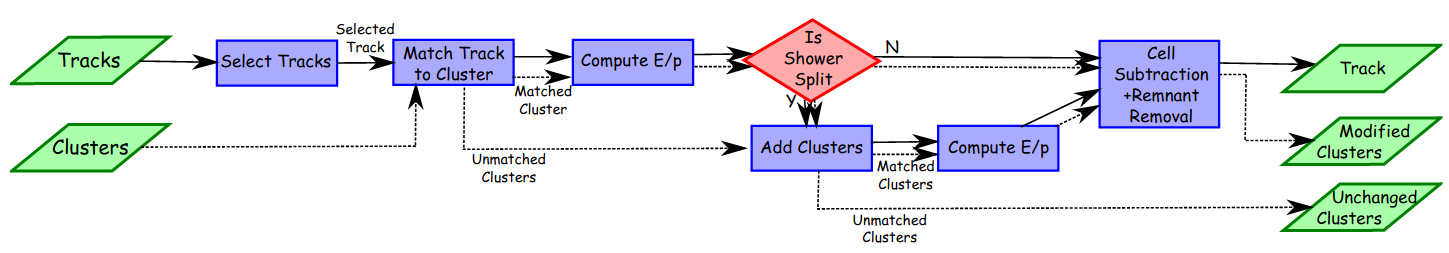
\includegraphics[width=1.\textwidth]{Ch4/Img/PFlow_Algo.png}
    \caption{A flow chart of how the particle flow algorithm proceeds, starting with track selection and continuing until the energy associated with the selected tracks have been removed from the calorimeter \cite{PFlow_Reco}.}
    \label{fig:Jet:JR:PFlowSketch}
\end{figure}
Similarly to EMTopo jets, the anti-$k_t$ algorithm with R=0.4 is used to reconstruct the PFlow jets. The algorithm takes as inputs the survived topo-clusters and the associated tracks that are matched to the hard scatter primary vertex. These criteria are applied to reject tracks originating from pile-up interaction \cite{Jet_pileUp}. \\
The PFlow is the jet type used in this thesis, while in the rest of this chapter the word "jet" refers to both EMTopo and PFlow.

\section{Jet Energy Calibration}
\label{Jet:Cal}
The resulting jets from the Monte Carlo simulation are needed to be calibrated such that, on average, the jet energy corresponds to that observed in the ATLAS detector. A jet calibration procedure is developed to calibrate the jet energy. This calibration proceeds in several sequential stages of calibration derived from a combination of Monte Carlo based methods, which correct the jet 4-momentum to the truth one in simulation, and $in-situ$ techniques that measure the difference in jet response between real and simulated data with residual correction applied to jet in data only.

\subsection{Jet Calibration Chain}
\label{Jet:Cal:chain}
 The first step in the calibration chain aims to recalculate the jet direction to point to the hard scatter primary vertex rather than the centre of the detector. This correction only affects the jet $\eta$ and resulting in a better $\eta$ resolution without changing the jet energy. Figure \ref{fig:Jet:Cal:chain} presents an overview of the ATLAS calibration scheme for jets.
\begin{figure}[htbp]
     \centering
     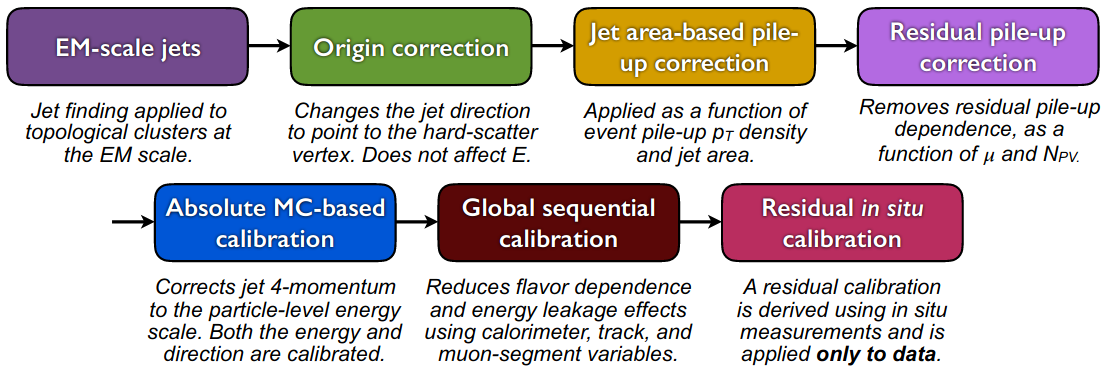
\includegraphics[width=0.8\textwidth]{Ch4/Img/calibration_chain.png}
     \caption{Calibration stages for jets. Other than the origin correction, each stage of the calibration is applied to the four-momentum of the jet \cite{JES_Sys_13_TeV}.}
     \label{fig:Jet:Cal:chain}
 \end{figure}

\subsubsection{Area-based and residual pile-up correction}
\label{Jet:Cal:chain:AreaPU}
This correction aims at subtracting the per-event energy excess due to in-time and out-of-time pile-up (Section \ref{chap2:LHC:PU}). The contribution from pile-up is evaluated from the median transverse energy density $\rho$. The correction is linked to jet area A and derived for jet within $|\eta|<$ 2 given the higher calorimeter occupancy in the forward region. An additional residual correction is derived to complete correction for the pile-up rate dependence remain after the area correction \cite{PileUp_Sub}. The dependence is seen on the number of reconstructed primary vertices $N_{PV}$, sensitive to the in-time pile-up, and the number of $pp$ interactions in the event $\mu$, sensitive to the out-of-time pile-up. The residual correction is derived as the difference between the reconstructed jet \pT and the truth jet \pT using a geometric reconstructed-truth matching with $\Delta R= $ 0.3. The area-based and pile-up correction is applied as:
\begin{equation}
    p_{\mathrm{T}}^{\mathrm{corr}}=p_{\mathrm{T}}^{\mathrm{reco}}-\rho A-\alpha\left(N_{\mathrm{PV}}-1\right)-\beta \mu,
\end{equation}
where $\alpha$ and $\beta$ are the slopes of the linear dependency of jet response respect to $N_{PV}$ and $\mu$.

\subsubsection{Absolute MC-based calibration}
\label{Jet:Cal:chain:JES}
This correction aims to correct, through a Monte Carlo based procedure, the reconstructed jet energy scale (JES) to the particle-level scale as well as the direction biases caused by the different calorimeter technologies and granularity. The average JES response is defined as the mean of a Gaussian fit to the core of the $R=E^{reco}/E^{truth}$ distribution in ($E^{truth}$, $\eta$) bins \cite{Old_JES, Old_JES_Sys}. A numerical inversion is used to parameterize the correction as a function of $E^{reco}$, the correction is applied as: 
\begin{equation}
    E_{JES}^{\mathrm{jet}}=\frac{E^{\mathrm{jet}}}{F(E^{\mathrm{jet}},\eta)},
\end{equation}
where $E_{JES}^{\mathrm{jet}}$ and $E^{\mathrm{jet}}$ are jet energy after and before the JES calibration, the $F(E^{\mathrm{jet}}, \eta)$ is the inverted jet response for a given (E,$\eta$) bin. A second correction is derived to account for a bias seen in the reconstructed jet $\eta$. The $\eta$ correction is computed as the difference between the reconstructed $\eta^{reco}$ and the truth $\eta^{truth}$ as a function of $E^{truth}$ and $\eta$. Similarly to JES correction, a numerical inversion is used to derive the correction in $E^{reco}$. This correction is evaluated on a multi-jet events sample. At this step, EMTopo (PFlow) jet is denoted EM+JES (PFlow+JES). Comparisons of the jet energy resolution measurement for PFlow+JES and EM+JES jets as a function of jet $p_T$ is shown in Figure \ref{fig:Jet:Cal:chain:JER}.
\begin{figure}[htbp]
    \centering
    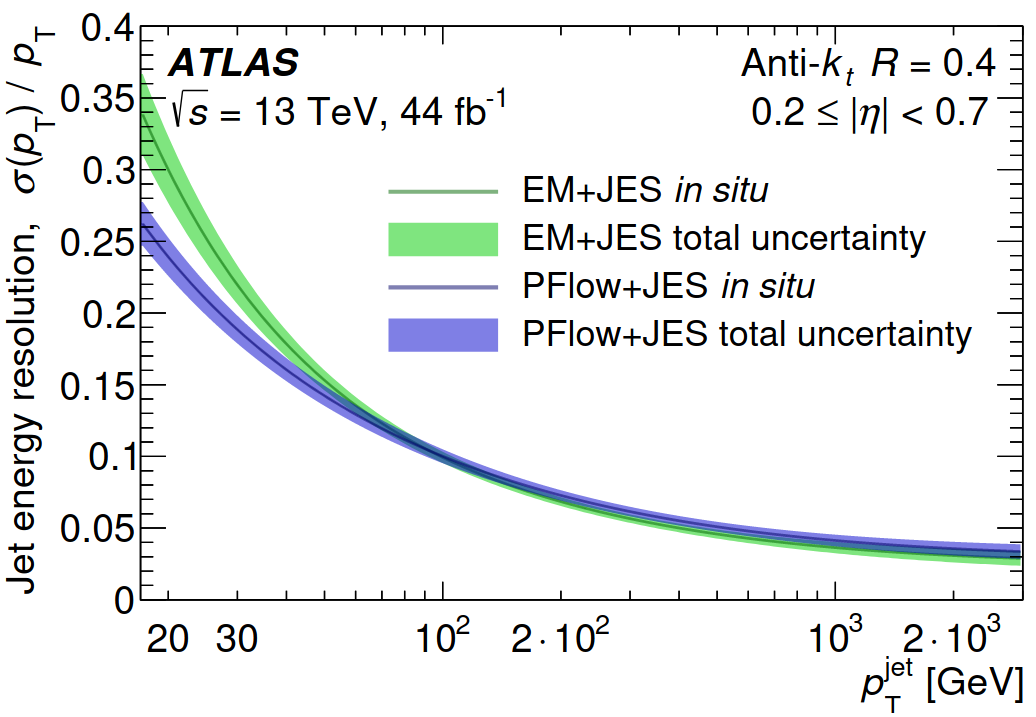
\includegraphics[width=0.6\textwidth]{Ch4/Img/Jet_Resolution_Topo_vs_PFlow.png}
    \caption{The relative jet energy resolution for fully calibrated PFlow+JES jets (green curve) and EM+JES jets (blue curve) as a function of $p_T$ jet.}
    \label{fig:Jet:Cal:chain:JER}
\end{figure}

\subsubsection{Global Sequential Calibration (GSC)}
\label{Jet:Cal:chain:GSC}
In this correction, the aim is to correct effects due to intrinsic properties of the jets not properly taken into account and the hadron composition yielded by the fragmentation process. The average particle composition and shower shape of a jet vary between initiating particles, most notably between quark- and gluon-initiated jets. The GSC uses five observables to improve the resolution of the JES jets. For each observable, an independent jet 4-momentum correction is derived as a function of $p_{T}^{truth}$ and $|\eta|$ by inverting the reconstructed jet response in Monte Carlo events. The effect of each correction is therefore to remove the dependence of the jet response on each observable while conserving the overall energy scale at the JES. No correlation between observables is taken into account. The five observables are:
\begin{enumerate}
    \item $f_{Tile0}$, the fraction of jet energy measured in the first layer of the hadronic Tile calorimeter.
    \item $f_{LAr3}$, the fraction of jet energy measured in the third layer of the electromagnetic LAr calorimeter.
    \item $n_{trk}$, the number of tracks with $p_T>$ 1 GeV associated with the jet.
    \item $\mathcal{W}_{trk}$, the average $p_T$-weighted transverse distance between the jet axis and all tracks of $p_T>$ 1 GeV associated to the jet.
    \item $n_{segments}$, the number of muon track segments associated with the jet.
\end{enumerate}

\subsubsection{Residual $in-situ$ calibration}
\label{Jet:Cal:chain:InSitu}
The last step of the jet calibration chain recovers the disagreement between real data and simulated Monte Carlo in the jet response coming from the imperfect detector simulation and mismodelling. The correction is extracted by balancing the jet $p_T$ against that of well-measured reference objects from Z+jets, $\gamma$+jets and dijet events. Figure \ref{fig:Jet:Cal:chain:InSitu} shows the final $in situ$ combination as a function of jet $p_T$. To complete the calibration, the inverse of the curve ($R_{MC}/R_{data}$) is taken as the scaling factor and applied to data. \\
Additional details on each calibration steps can be found in the Reference \cite{JES_Sys_13_TeV}. \\
Figure \ref{fig:Jet:Cal:chain:JER} demonstrates the performance of PFlow at low jet \pT coming from combining calorimeter and tracking information as well as the low threshold on track \pT, for high jet \pT the performances of both EMTopo and PFlow are comparable. 
\begin{figure}[htbp]
    \centering
    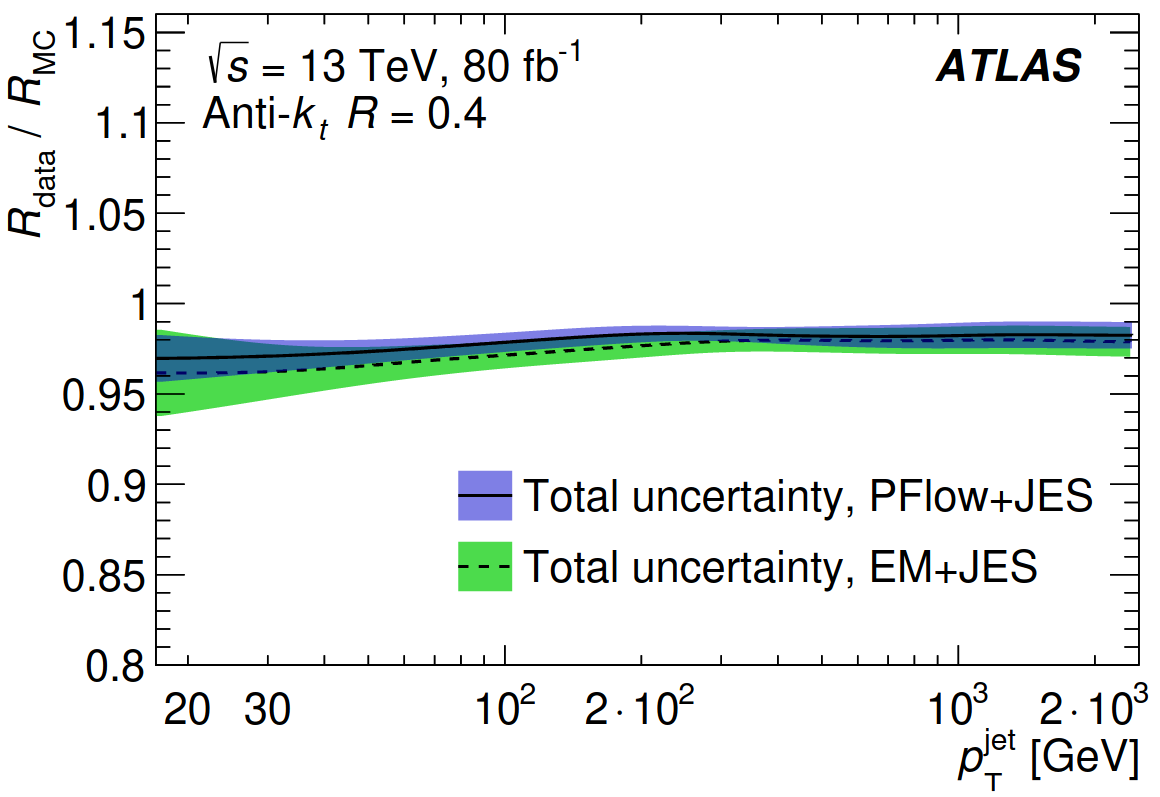
\includegraphics[width=0.6\textwidth]{Ch4/Img/Jet_MC_Data_Ration.png}
    \caption{Ratio of the PFlow+JES (blue curve) and EM+JES (green curve) jet response in data to that in the nominal Monte Carlo event generators as a function of $p_T$ jet.}
    \label{fig:Jet:Cal:chain:InSitu}
\end{figure}

\section{Jet Tagging : Pile-up and flavour taggings}
\label{Jet:Tag}
Jets coming from pile-up (PU) vertices can have a disastrous impact on physics analysis, by leading to fake jets and therefore biasing the event selection. PU jets are coming either from hard-scatter interaction from a primary vertex that is not the vertex from which the process of interest is arising, defining the most frequent type of jet QCD-PU, or from interactions that are not related to the initial one defining the stochastic PU. Removing PU jets has a critical importance \cite{Tagging_2013, Tagging_2014}. $Jet\ Vertex\ Tagger$ (JVT) and $forward \ Jet \ Vertex\ Tagger$ (fJVT) are two algorithms used to identify hard-scatter (HS) and PU jets \cite{JVT_2014, fJVT}. In addition to PU jets, identifying the initial nature of the jets is needed for specific analyses such as the \HHyybb which require their jets to be originating from the $b$-quark fragmentation instead of being from gluons or other quarks. For that specific $b$-tagging algorithm designed to discriminate between $b$-jets and other jets \cite{Light_Quark_Tagger}. This section includes details on each tagging algorithm. 

\subsection{Jet Vertex Tagging (JVT) algorithms}
\label{Jet:Tag:JVT}

\subsubsection{JVT}
\label{Jet:Tag:JVT:JVT}
Jet can be matched to its vertex origin within $|\eta|<$ 2.5 (the ID acceptance) where the tracking information is available. Information from this matching is the main ingredient of the JVT algorithm \cite{JVT_Perf}. A global JVT discriminant is constructed from two track-based variables using $k$-nearest-neighbour algorithm \cite{kNN}. The two variables are defined as: 
\begin{equation}
    corrJVF=\frac{\sum_{k} p_{\mathrm{T}}^{ {track
    }_{k}}\left(\mathrm{PV}_{0}\right)}{\sum_{l} p_{\mathrm{T}}^{{track
    }_{l}}\left(\mathrm{PV}_{0}\right)+\frac{p_{\mathrm{T}}^{\mathrm{PU}}}{k . n_{\ {tracks }}^{\mathrm{PV}}}},
\end{equation}

\begin{equation}
    R_{p_{\mathrm{T}}}=\frac{\sum_{k} p_{T}^{\mathrm{track}_{k}}\left(\mathrm{PV}_{0}\right)}{p_{\mathrm{T}}^{j e t}},
\end{equation}
The  $\sum_{k} p_{\mathrm{T}}^{{track}_{k}}\left(\mathrm{PV}_{0}\right)$ term, appearing in both formulas, represents the scalar sum of tracks $p_T$ originating from the hard scattered vertex and associated to a jet, corrJVF also uses a similar term for PU vertices $p_{\mathrm{T}}^{\mathrm{PU}}=\sum_{n \geq 1} \sum_{l} p_{\mathrm{T}}^{\mathrm{track}_{l}}\left(\mathrm{PV}_{n}\right)$  where PU vertices are noted as $\mathrm{PV}_{n}$, $\frac{1}{k . n_{tracks }^{\mathrm{PU}}}$ where k=0.01 is a correction factor used to correct the behaviour from linear increase with the number of tracks. For both EMTopo and PFlow the JVT is built similarly, while WPs are defined differently for the two types of jets given the fact that PFlow has built-in pileup jet suppression in its reconstruction algorithm. For EMTopo three WPs are defined (Loose, Medium and Tight) and only two WPs (Medium and Tight) are defined for PFlow jets. Figure \ref{fig:Jet:Tag:JVT} shows the JVT reconstructed variable as well as the fake rate efficiency for JVF, $R_{p_T}$, corrected JVF and the combined JVT discriminate variables.
\begin{figure}[htbp]
    \centering
    \subfloat[][]{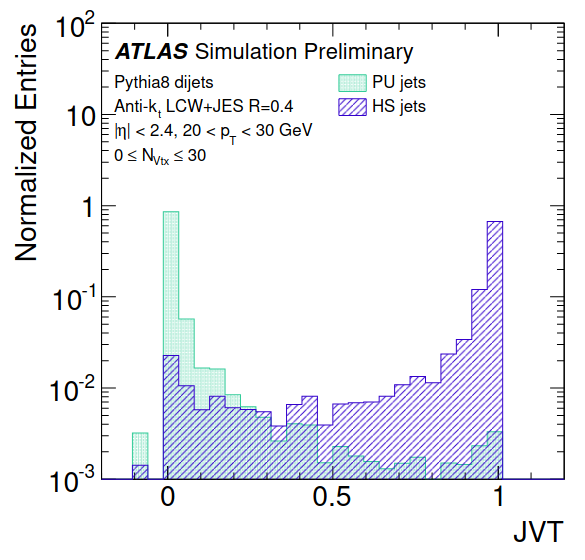
\includegraphics[width=.5\textwidth]{Ch4/Img/JVT.png}}
    \subfloat[][]{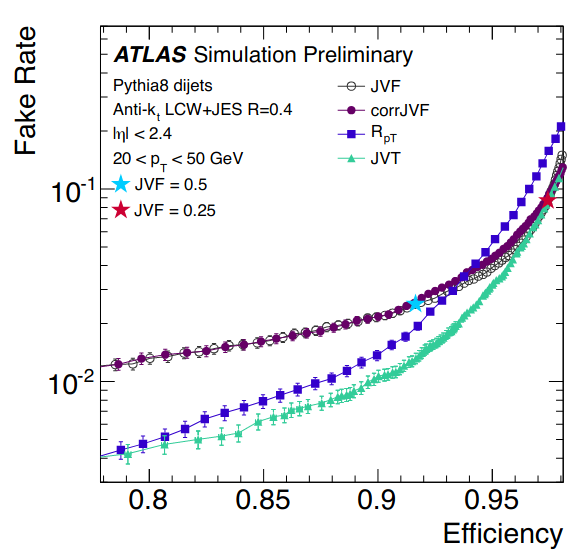
\includegraphics[width=.5\textwidth]{Ch4/Img/JVT_Eff.png}} 
    \caption{(a) Comparative distribution, scaled to unity, of JVT for truth-matched HS and PU. (b) PU-jet fake rate as a function of the HS-jet efficiency for cuts on the JVT discriminant and JVT input variables. The performance is compared to that of the JVT inputs, corrJVF and $R_{p_T}$, as well as that of the no corrected JVF.}
    \label{fig:Jet:Tag:JVT}
\end{figure}

\subsubsection{fJVT}
\label{Jet:Tag:JVT:fJVT}
For jets outside the ID acceptance ($|\eta|>$ 2.5), the JVT can not be used due to the absence of tracking information. The fJVT algorithm procedure is quite different from the JVT since it starts by selecting central QCD PU jets and associate them with the corresponding vertex. Then for each vertex i, the missing transverse momentum $-\vec{p}_{T, i}$ is computed, averaging the jet and track component, as:
\begin{equation}
    -\vec{p}_{T, i}=\frac{1}{2}\left(k \cdot \sum_{tracks \in P V_{i}} \vec{p}_{T}^{track }+\sum_{jets \in PV_{i}} \vec{p}_{T}^{jet}\right)
\end{equation}
where k=2.5 is a factor to account for intrinsic differences between the jet and tracks terms. The fJVT discriminant is therefore for a given jet is defined as:
\begin{equation}
    fJVT = max(fJVT_i) = max(\frac{-\vec{p}_{T, i} \cdot \vec{p}_{T}^{j e t}}{\vec{p}_{T}^{j e t} \cdot \vec{p}_{T}^{j e t}})
\end{equation}
where $fJVT_i$ is the jet fJVT to the vertex i. Figure \ref{fig:Jet:Tag:JVT:fJVT} shows the fJVT discriminant tends to have large values for QCD pileup jets, while the distribution for hard-scatter jets falls steeply.
\begin{figure}[htbp]
    \centering
    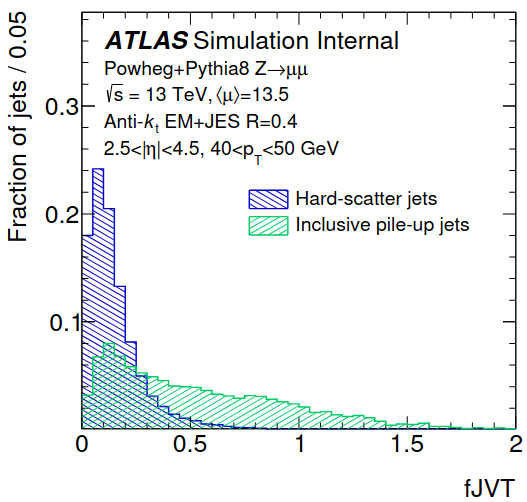
\includegraphics[width=0.5\textwidth]{Ch4/Img/fJVT.png}
    \caption{The fJVT distribution for hard-scatter (blue) and pileup (green) forward jets.}
    \label{fig:Jet:Tag:JVT:fJVT}
\end{figure}
It is important to note that the fJVT discriminant is only clearly defined for QCD PU jets, as opposed to stochastic pileup jets. To be able to select stochastic jets, fJVT is accompanied by an additional requirement on jet timing. Two fJVT working point are defined Loose WPs which correspond to fJVT$<$ 0.5 and a Tight one with fJVT$<$ 0.4, their efficiencies are shown in Figure \ref{fig:Jet:Tag:JVT:Eff}.
\begin{figure}[htbp]
    \centering
    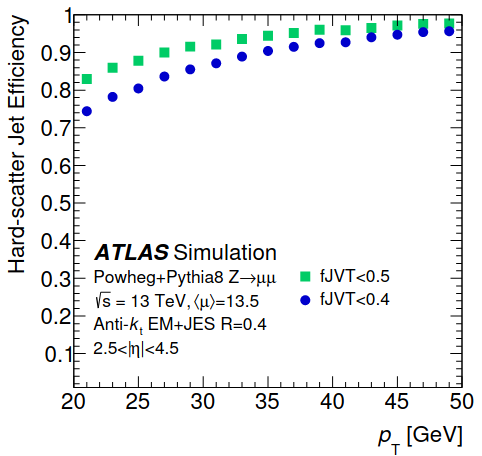
\includegraphics[width=0.5\textwidth]{Ch4/Img/fJVT_Eff.png}
    \caption{Efficiency for hard-scatter jets as a function of the forward jet $p_T$.}
    \label{fig:Jet:Tag:JVT:Eff}
\end{figure}
An additional improvement in the fJVT performances is achieved by combining fJVT, timing, and jets shapes and kinematics information using machine learning techniques \cite{Louis_Thesis}. 

\subsection{\texorpdfstring{$b$}-jet tagging}
\label{Jet:Tag:Dlr}
The identification of jets originating from \bq-quark decay, called \bq-tagging, is important for all analyses involving \bq-quark in their final state, such as the analysis presented in this thesis \HHyybb. The \bq-jet identification relies of identifying the secondary displaced vertex given the long lifetime of \bq-hadrons $\sim$ 491.1 $\mu$m compare to $c$-jet or gluon- (light) jets. $B$-tagging algorithms are designed to discriminate between \bq-jets and other types. They are based on several low-level algorithms that exploit information from reconstructed tracks in the ID and MS which are combined by a high-level \bq-tagging algorithm into a single discriminate variable used at the analysis level. Two high-level \bq-tagging are developed MV2 which is based on the BDT, and the DL1 based on neural networks (NNs), both algorithms use almost the same input from low-level algorithms except for the DL1 that include additional inputs related to the semi-leptonic decay of heavy-flavoured hadrons topology. Each low-level flavour tagging algorithm focuses on different flavour-sensitive information, deriving different sets of variables based on the impact parameter algorithms of tracks in jets (IPs), the presence and properties of an inclusive secondary vertex (SV) and the reconstruction of the \bq- and $c$-hadron multi-vertices chain topology (JetFitter):
\begin{itemize}
    \item Impact Parameter based algorithms: use a log-likelihood ratio (LLR) to separate tracks associated with jets according to whether or not they are compatible with the primary vertex hypothesis. The LLR is computed as the sum of per-track contributions $\sum_{i=1}^{N}log(p_b/p_u)$ where N is the number of tracks and $p_b$, $p_u$ are the probability density functions (PDFs) for the $b$- and light-jet hypotheses respectively. The algorithms do not take into account tracks correlation \cite{IP,IP2}. 
    \item Secondary Vertex finding: explicitly reconstructs an inclusive displaced secondary vertex within the jet. All track pairs within a jet are tested for a two-track vertex hypothesis using a $\chi^2$. Two-track vertices are discarded if they were likely to originate from the decay of a long-lived particle, photon conversions or hadronic interactions with the detector material \cite{SV}.
    \item Decay Chain Multi-Vertex algorithm (JetFitter): exploits the topological structure of weak $b$- and $c$-hadron decays inside the jet and tries to reconstruct the full \bq-hadron decay chain. A Kalman filter is used to find a common line on which the primary vertex and the bottom and charm vertices lie, approximating the \bq-hadron flight path, as well as their positions \cite{JetFitter}.
\end{itemize}
Outputs from these algorithms construct input to MV and DL1. Many variations of DL1 exist with different NN configurations and additional inputs. The DL1r adopted in the work of this thesis as well as ATLAS publications also include input from a Recurrent Neural Network (RNN) based IP algorithm to consider the correlation among tracks \cite{DL1r}. The final discriminant for \bq-tagging efficiency is calculated as:
\begin{equation}
    \mathrm{DL} 1=\ln \left(\frac{\mathrm{p}_{b}}{\mathrm{f}_{c-\mathrm{jets}} \cdot \mathrm{p}_{c}+\left(1-\mathrm{f}_{c-\mathrm{jets}}\right) \cdot \mathrm{p}_{light-flavour }}\right),
    \label{b-jet}
\end{equation}
where $p_b$, $p_c$ and $p_{light-flavour}$ are the NN outputs probabilities that the jet is a \bq-jet, $c$-jet or light-jet respectively. $f_{c-jets}$ is the $c$-jet fraction taken into account, which can be tuned separately according to physics analysis needs. \\  
For both MV2 and DL1, 4 WPs are computed for different \bq-tagging efficiencies. The WPs are defined as a fixed cut or \pT dependent cut on the final discriminant variable (Eq. \ref{b-jet}) and labelled with the corresponding integrated efficiency on \bq-jets. The working points are 85\%, 77\%, 70\% and 60\%. Figure \ref{fig:Jet:Tag:Dlr:Eff} shows a comparison of performances for 2018 recommended versions of MV2 and DL1, and 2019 DL1r optimization. The 2019 DL1r shows a significant improvement over other algorithms. Figure \ref{fig:Jet:Tag:Dlr:Eff_77} shows the efficiency of identifying \bq-jets as a function of jet \pT for 77\% WP requirement, for 2018 recommended versions of MV2 and DL1, and 2019 DL1r optimization \cite{Btag_Perf}. 
\begin{figure}[htbp]
    \centering
    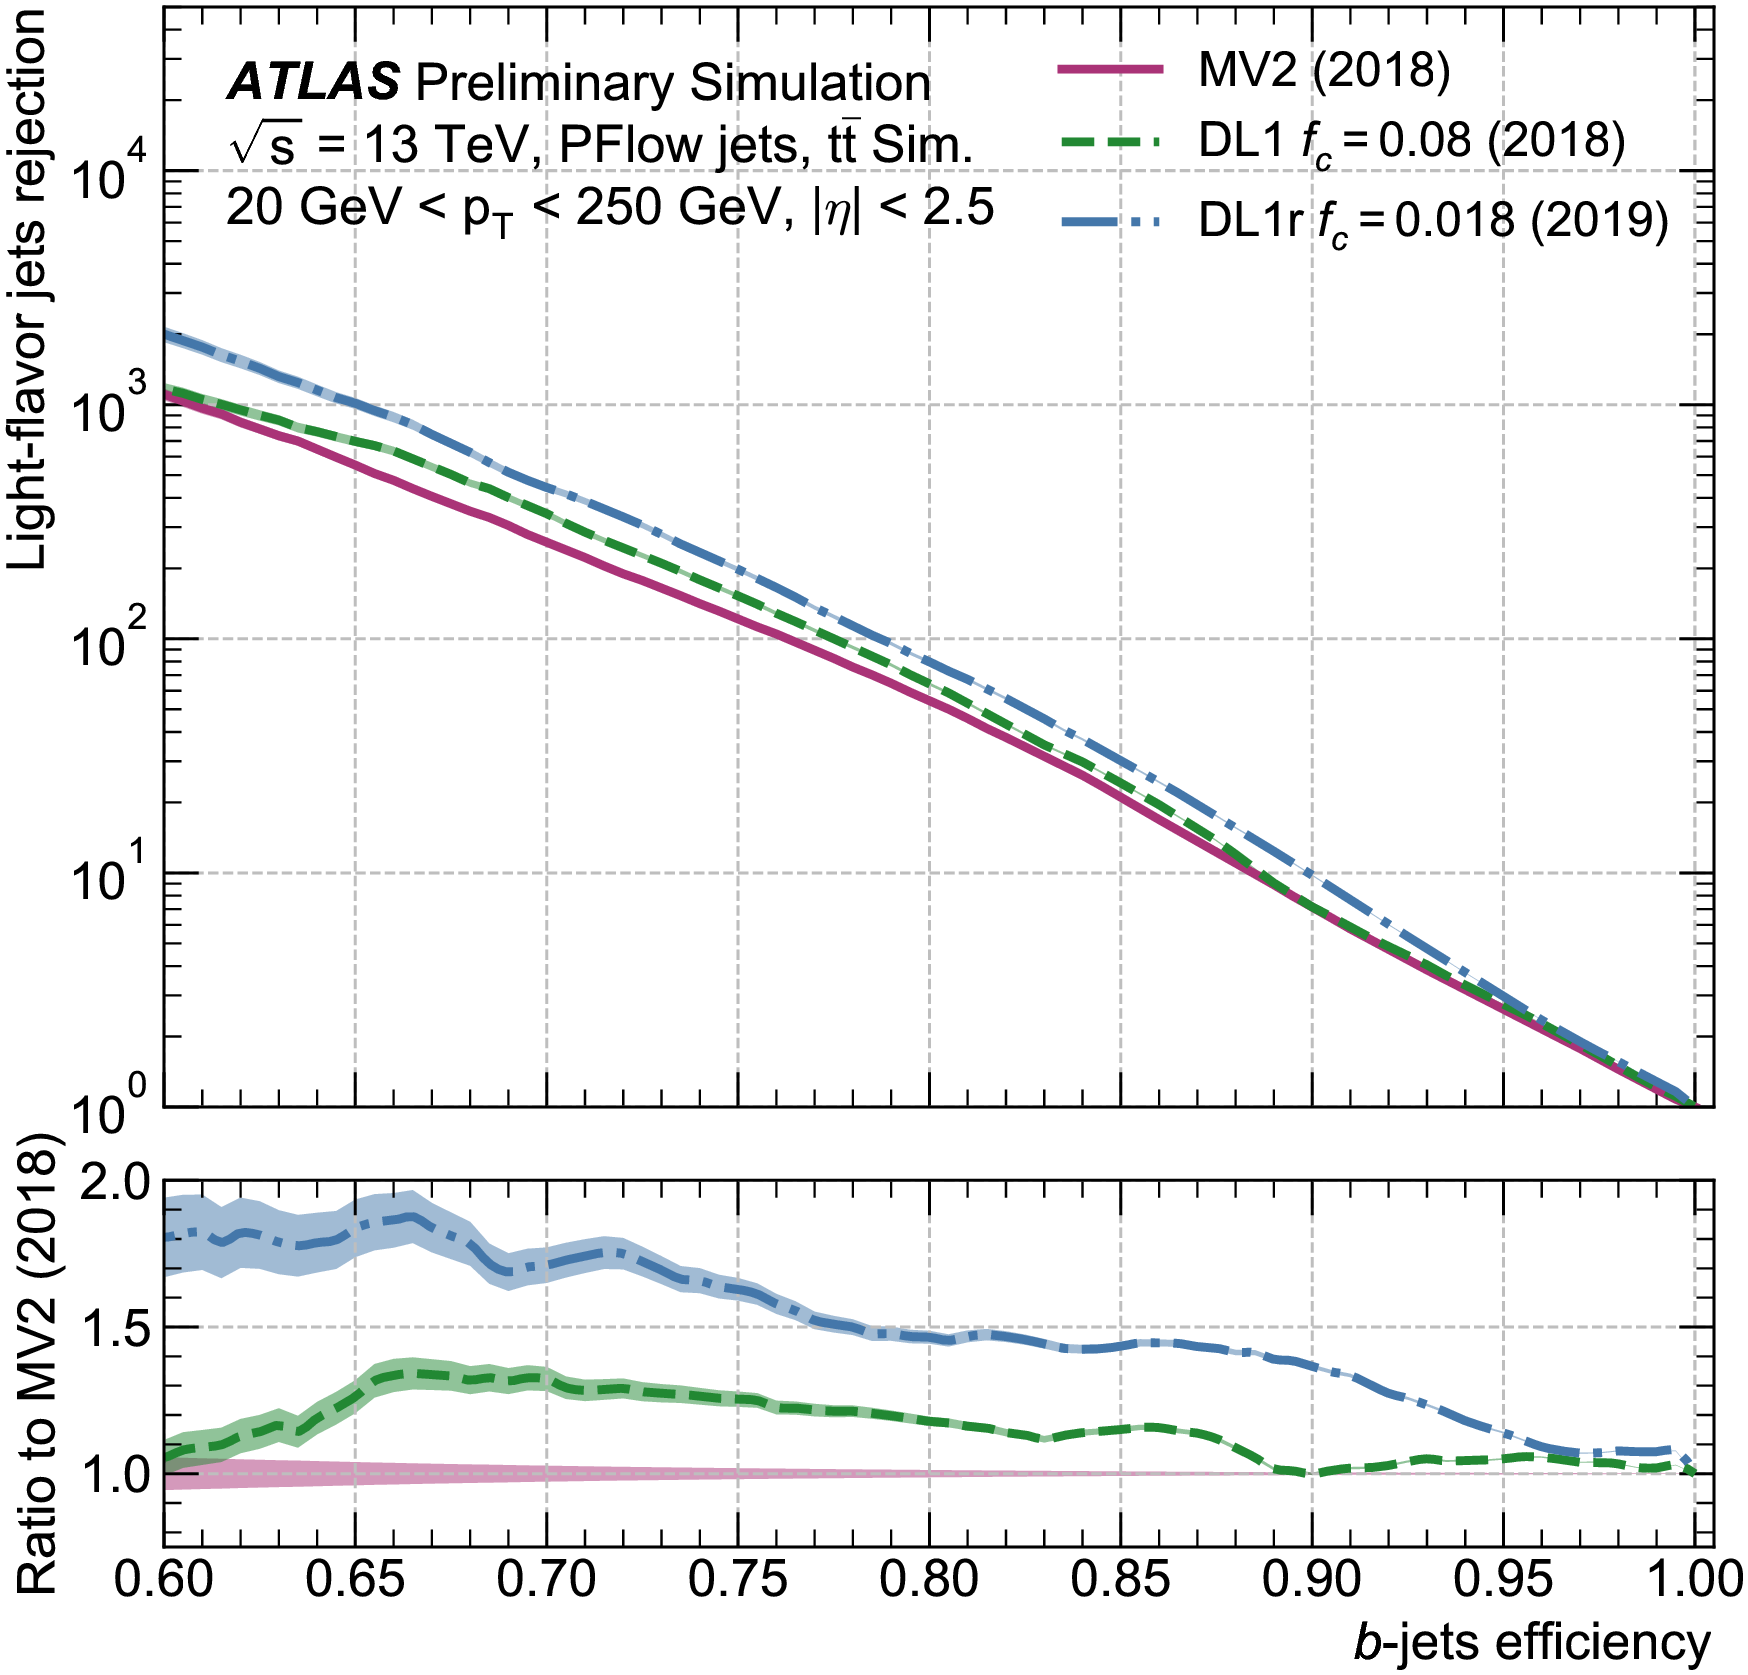
\includegraphics[width=0.5\textwidth]{Ch4/Img/b_jet_Eff.png}
    \caption{ROC curves for 2018 recommended versions of MV2 and DL1, and 2019 DL1r optimization. The x-axis corresponds to the b-jet efficiency, while the y-axis corresponds to light-flavor jets rejection. The shaded bands represent the statistical uncertainty.}
    \label{fig:Jet:Tag:Dlr:Eff}
\end{figure}
\begin{figure}[htbp]
    \centering
    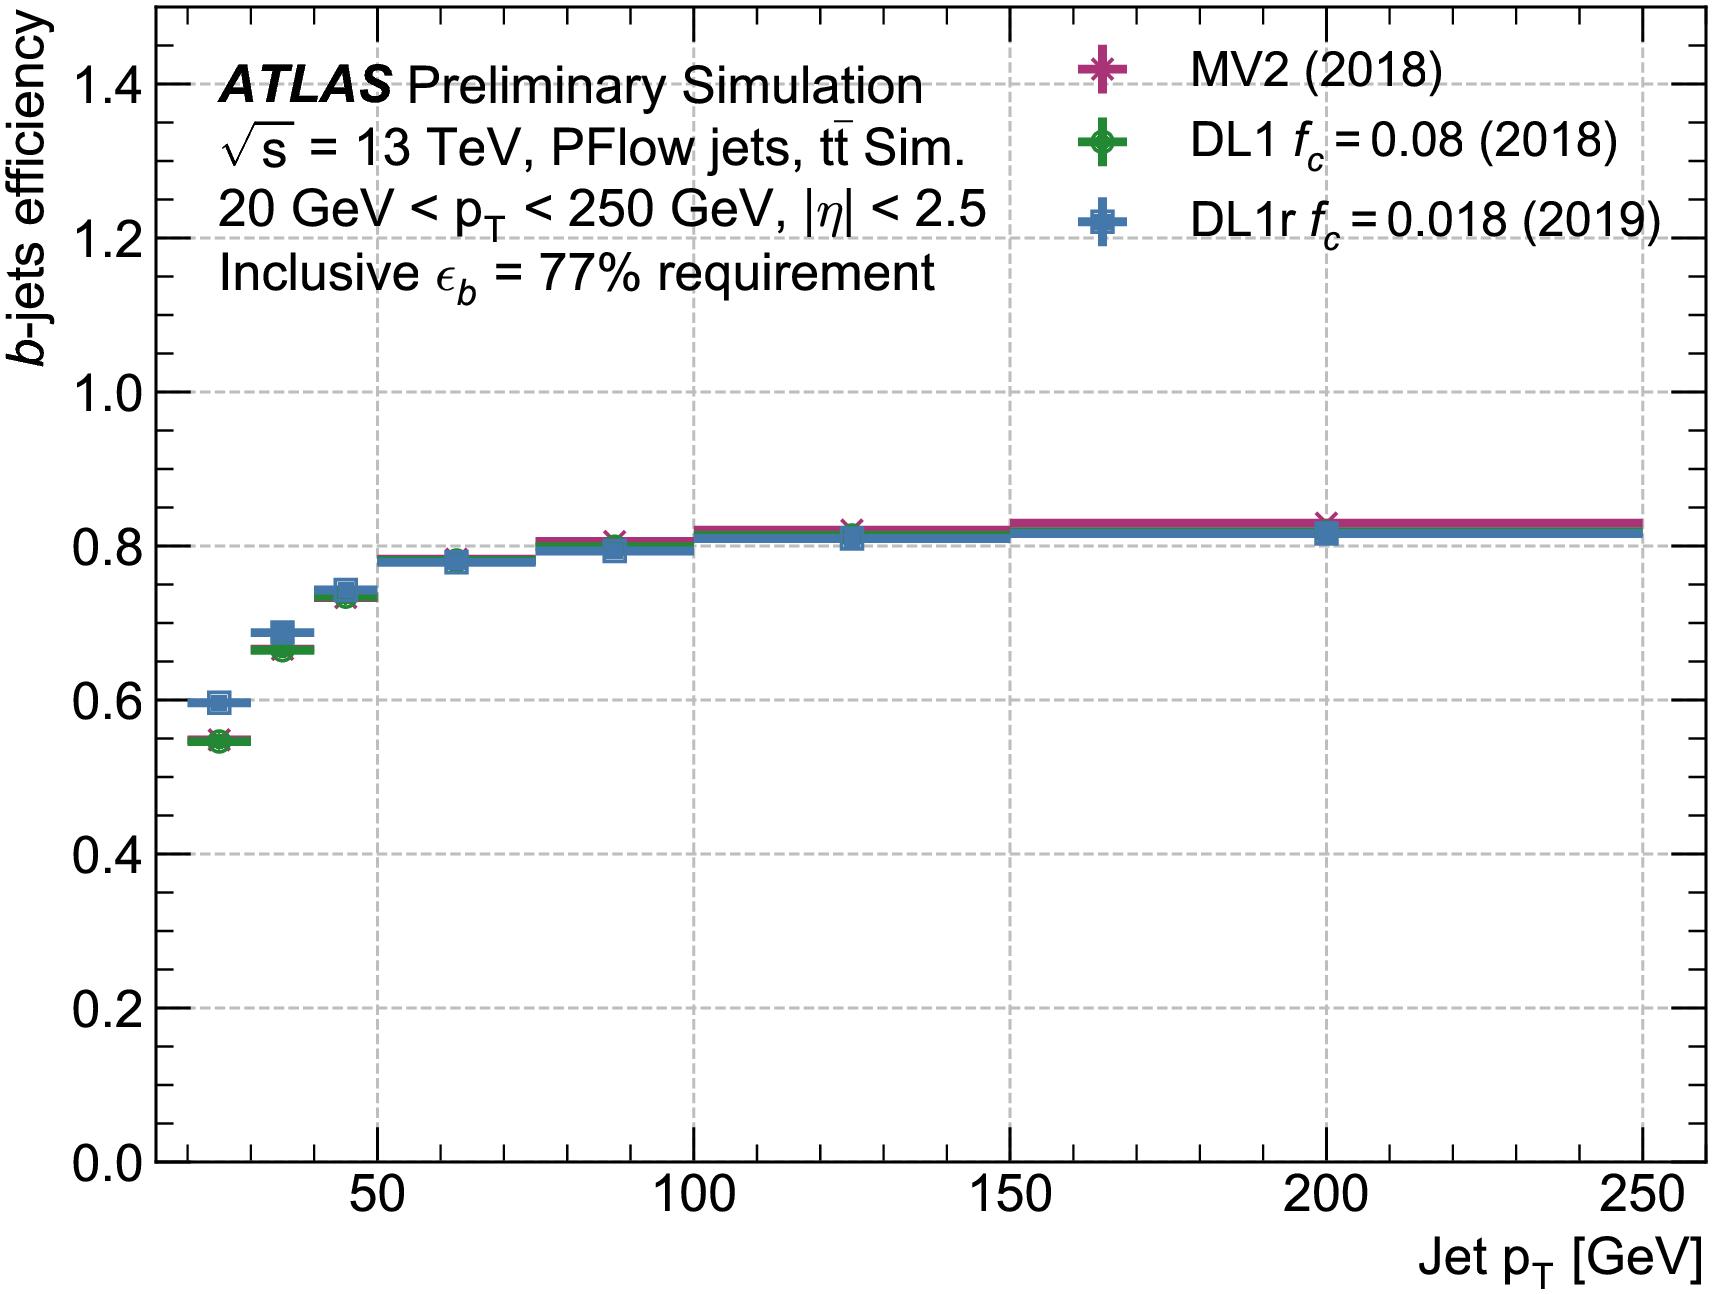
\includegraphics[width=0.5\textwidth]{Ch4/Img/b_jet_Eff_77.png}
    \caption{Efficiency of identifying b-jets as a function of jet pT for an inclusive 77\% efficiency requirement, for 2018 recommended versions of MV2 and DL1, and 2019 DL1r optimization.}
    \label{fig:Jet:Tag:Dlr:Eff_77}
\end{figure}

\section{\texorpdfstring{$b$}-jet energy calibration}
\label{Jet:Cal:BCal}
The default JES calibration (Section \ref{Jet:Cal:chain:JES}) applied to all jets is a correction optimised on multi-jet events which are mainly light-quark jets. This correction is not optimal for \bq-jets due to:
\begin{itemize}
    \item large \bq-quark mass which reduces the boost of the jet and, as consequence, a larger fraction of the jet particles lay outside the usual jet cone leading to out-of-cone radiation.
    \item larger semi-leptonic branching ratio of \bq-hadrons which produce elusive neutrino.
\end{itemize}
Figure \ref{fig:Jet:Cal:BCal:bJet} illustrates these statements through the schematic of a \bq-jet. To overcome this issue, a step-by-step approach, firstly developed in VH($H\rightarrow b\bar{b}$) analysis demonstrates a potential improvement \cite{Vhbb}, the first correction called "$\mu$-in-jet" includes soft muon in the jet to address the semi-leptonic decays of \bq-hadrons inside \bq-jet. The second correction called "$p_T$Reco" corrects \bq-jets for the neutrino presence in the semi-leptonic decay and out-of-cone radiation effect by introducing a global correction factor to correct the jet transverse momenta. The developed approach in VH(bb) is computed only for EMTopo \bq-jets from the signal VH(bb) simulated events. To generalize this correction to any channel with \bq-jets in the final state its amplitude is computed from \bq-jets produced in $t\bar{t}$ simulated event for both EMTopo and PFlow jets. This correction is added as an additional step to the calibration chain already mentioned above (Figure \ref{fig:Jet:Cal:BCal:Chain}).
\begin{figure}[htbp]
    \centering
    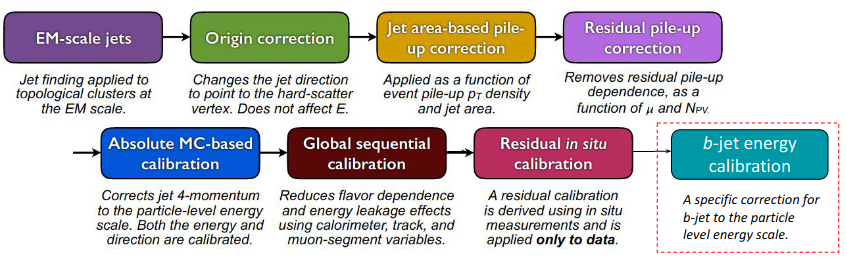
\includegraphics[width=0.8\textwidth]{Ch4/Img/b_jet_chain.png}
    \begin{tcolorbox}[colback=black!5!white,colframe=white!75!black]
    \caption{Calibration stages for jets including \bq-jet energy correction.}
    \label{fig:Jet:Cal:BCal:Chain}
    \end{tcolorbox}
\end{figure}
\begin{figure}[htbp]
    \centering
    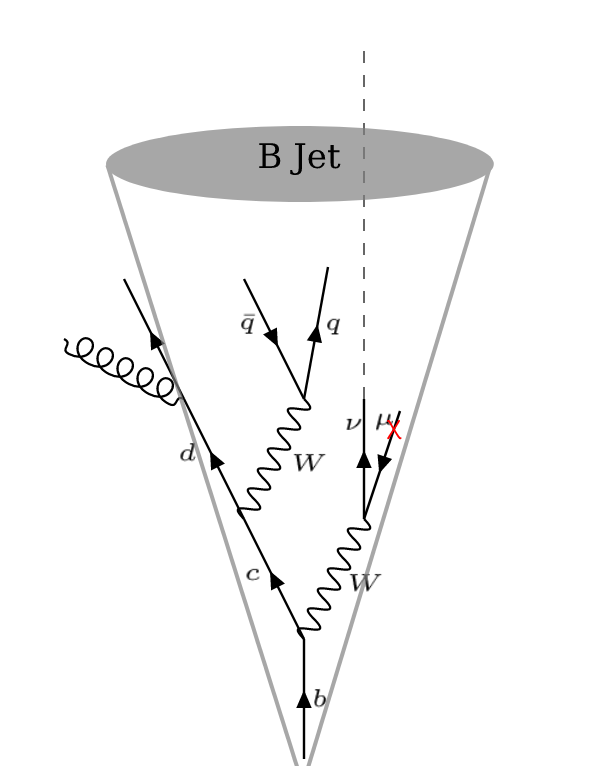
\includegraphics[width=0.4\textwidth]{Ch4/Img/b-jet.png}
    \begin{tcolorbox}[colback=black!5!white,colframe=white!75!black]
    \caption{Example of a \bq-jet.}
    \label{fig:Jet:Cal:BCal:bJet}
    \end{tcolorbox}
    
\end{figure}

\subsection{\texorpdfstring{$\mu$}-in-jet correction}
\label{Jet:Cal:BCal:MuInJet}
The decays of $B$ and $D$ hadrons produce each three type of leptons with a branching ratio of 11\%. These leptons are usually mixed with other particles within jets. For electrons and taus, their identification efficiency is low and, as a consequence, will not be flagged as semi-leptonic and their energies are fully included in the jet reconstruction as mentioned in Section \ref{Jet:JR}. The energy coming from their associated neutrinos will be mixed with $p_T$Reco. Instead, the muon is a minimum ionizing particle, depositing very little energy in the calorimeter. To correct for the semi-lepton decay, the four-vector momenta of a muon found inside the jet is added to the four-vector momenta of the jet. To select the associate muon to the jet, selection criteria, listed in Table \ref{tab:Jet:Cal:BCal:MuInJet:Sel}, were defined.
\begin{table}[htbp]
    \centering
    \begin{tabular}{cc}
       \hline\hline
        Criteria & Selection \\
        \hline
        $p_T$ & $>$ 4 GeV \\
         ID & Medium \\
         $\Delta R$ &  $<$VR\\
         \hline
         \hline
    \end{tabular}
    \caption{Muon selection requested for $\mu$-in-jet correction}
    \label{tab:Jet:Cal:BCal:MuInJet:Sel}
\end{table}
$\Delta R$ represents distance between jet and muon axis. VR is computed using the formula:
\begin{equation}
    \mathrm{min}(0.4, 0.04+10/p_T)
\end{equation}
with muon \pT in GeV. Instead of a 0.4 fixed cut on $\Delta R$, a variable cut is applied which takes into account the fact that jet boost reduces the angular distance of the muon. If more than one muon is identified, only the one with the highest transverse momentum (closest) is used. Such muons are found for 12\% of the b-tagged jets. The 4-vector momenta associated with the muon passing the selection is added back to jet one after having subtracted the estimated energy deposited in the calorimeter. The associated jets with a muon are labelled as "semi-leptonic" while others are labelled "hadronic".

\subsection{\texorpdfstring{$p_T$}Reco correction}
\label{Jet:Cal:BCal:pTReco}
On top of $\mu$-in-jet correction, a global \pT dependent scale factor is applied to the jet 4-vector to correct for the presence of neutrino in semi-leptonic decays and out-of-cone radiation. The relevant target is the particle-level \texttt{TruthWZ} jets container, which contains reconstructed jets with the same reconstruction algorithm ($AntiK_t$), using all stable hadrons and non-isolated muons and neutrinos. To generalize the correction and make it signal independent and used by any analysis with $b$-jet in the final state, the correction factor is derived from a $t\bar{t}$ sample. It is binned in $ln(p_T)$ of reconstructed jet up to 400 GeV. The log scale is used because of the exponential shape of \pT spectrum and to provide a smooth distribution for interpolation. The scale factor is computed separately for semi-leptonic and hadronic jets and evaluated as the mean of the distribution of the ratio between reconstructed $b$-jet \pT and the corresponding \texttt{TruthWZ} jet \pT, matched within $\Delta R < 0.3$ for the given \pT bin. For each $b$-tagged jet, the 4-vector is scaled by the scale factor computed using a linear interpolation by \texttt{TH1::Interpolate(ln(\pT))} function. The correction is derived for each jet reconstruction algorithms EMTopo or PFlow and each $b$-tagging algorithms MV2 or DL1r. Figure \ref{fig:Jet:Cal:BCal:pTReco} shows the correction factor distribution for different DL1r jet labels and reconstruction algorithms. 
\begin{figure}[htbp]
   \centering
   \subfloat[][]{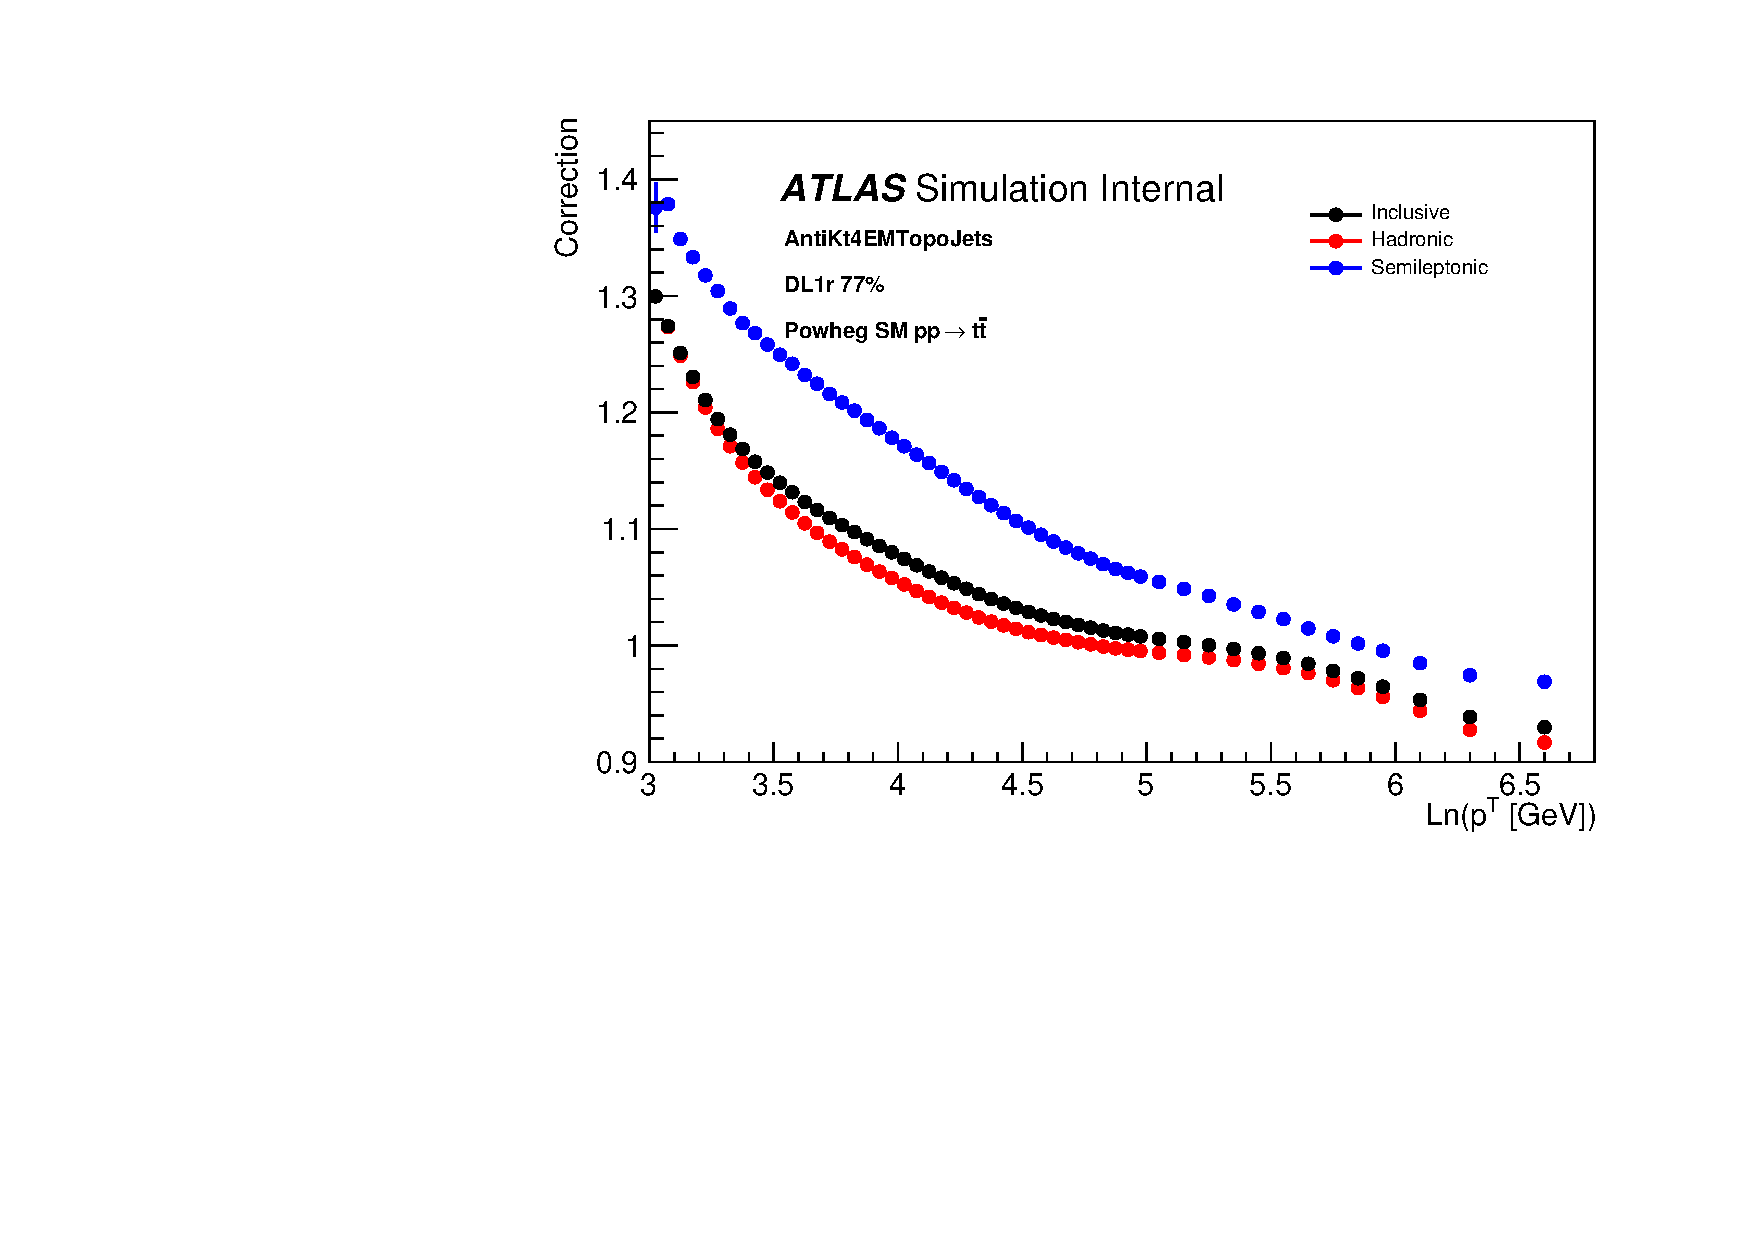
\includegraphics[width=.48\textwidth]{Ch4/Img/PtRec_AntiKt4EMTopoJets.pdf}}\quad
   \subfloat[][]{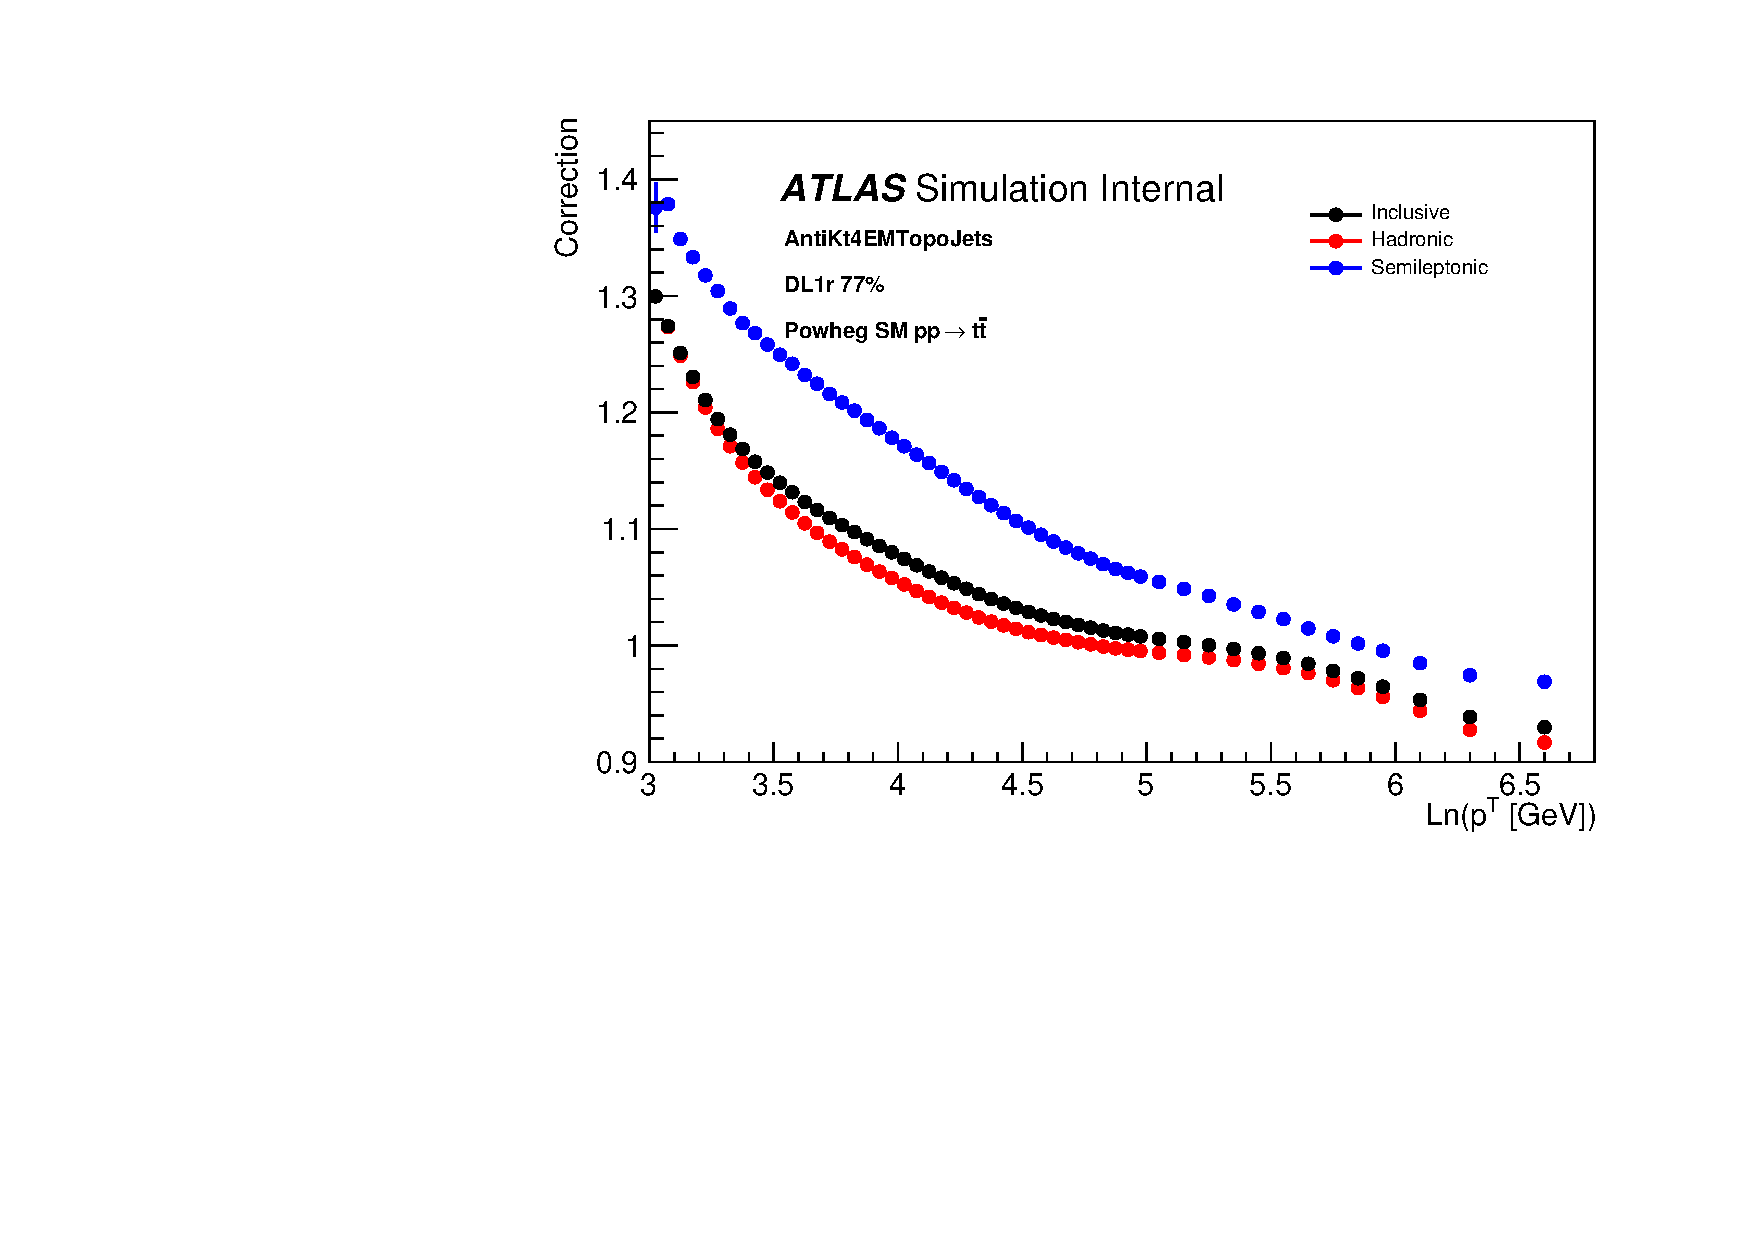
\includegraphics[width=.48\textwidth]{Ch4/Img/PtRec_AntiKt4EMTopoJets.pdf}}
   \begin{tcolorbox}[colback=black!5!white,colframe=white!75!black]
   \caption{$p_T$Reco correction distribution for (a) topological cluster jets (b) particle flow jets, \bq-tagging 77\% WP is applied with DL1r algorithm.}
   \label{fig:Jet:Cal:BCal:pTReco}
   \end{tcolorbox}
   
\end{figure}
Figure \ref{fig:Jet:Cal:BCal:pTReco} shows that :
\begin{itemize}
    \item EMTopo hadronic factor is much higher than the one for PFlow at low jet \pT ($\sim$ 10\%). This is explained by the fact that PFlow combines tracking, soft activity and calorimetric information to reconstruct the jet, so it includes low \pT (\pT $>$ 0.5 GeV) tracks that do not reach the calorimeter, which helps to reduce the out-of-cone effects, as mentioned in Section (\ref{Jet:JR}). 
    \item The presence of neutrino in semi-leptonic jets explains the higher correction compared to hadronic jets (up to $\sim$ 10\% for low \pT jet).
    \item At high jet \pT the distribution on the ratio between the reconstructed \pT and the truth one has a large tail below 1 which leads to a correction factor below 1 indicating that the reconstructed jet \pT is higher than the truth. This can be explained by the fact that at high \pT the \bq-quark fragmentation at truth level gives two closest jets, only one is identified as $b$-jet, but at reconstruction level, both are reconstructed as a single $b$-jet.
\end{itemize}

\subsection{\texorpdfstring{$b$}-jet energy correction improvement}
\label{Jet:Cal:BCal:Result}
Figure \ref{fig:Jet:Cal:BCal:Result:E}, shows the maximum possible gain in $b$-jet energy resolution in $t\bar{t}$ sample (used to compute the $p_{T}$Reco correction). The energy resolution is improved by 40\% (20\%) for high (low) energy for semi-leptonic jet, and about 20\% (5\%) for high (low) energy for hadronic jet. Almost similar improvement is observed for both jet types (EMTopo and PFlow).
\begin{figure}[htbp]
   \centering
   \subfloat[][]{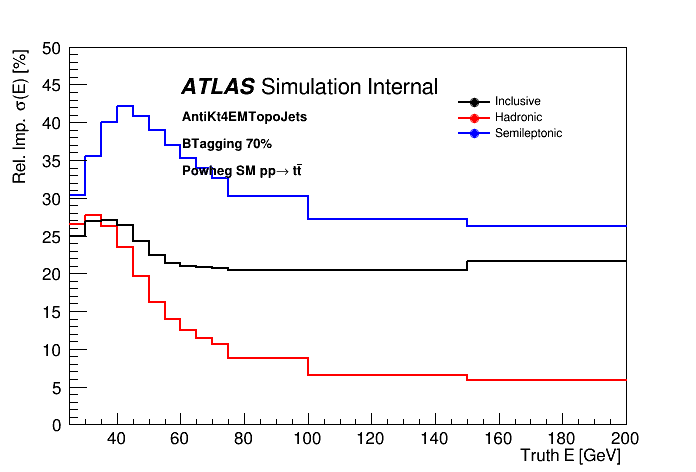
\includegraphics[width=.48\textwidth]{Ch4/Img/E_AntiKt4EMTopoJets.png}}\quad
   \subfloat[][]{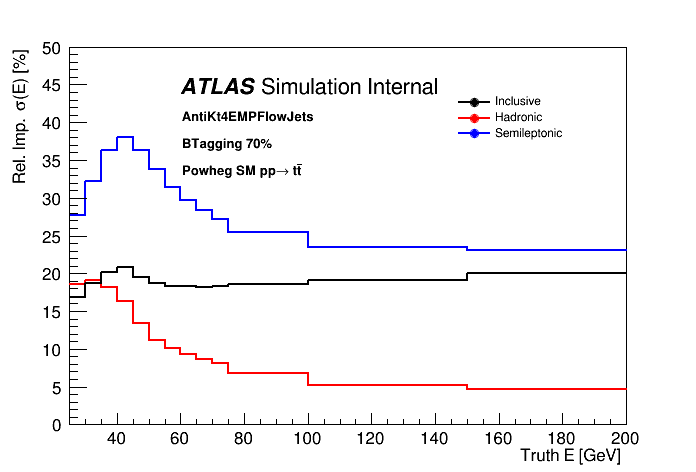
\includegraphics[width=.48\textwidth]{Ch4/Img/E_AntiKt4EMPFlowJets.png}}
   \begin{tcolorbox}[colback=black!5!white,colframe=white!75!black]
   \caption{Relative energy resolution improvement after \bq-jet energy calibration in bin of truth energy for $t\bar{t}$ using (a) topological cluster jets (b) particle flow jets.}
    \label{fig:Jet:Cal:BCal:Result:E}
   \end{tcolorbox}

\end{figure}

\subsubsection{Improvement on $H\rightarrow\bar{b}b$}
 The power of \HHyybb is coming from the $H\rightarrow\gamma\gamma$ part wish has a very narrow peak helping in rejection a huge amount of the continuum background by defining a narrow window on $m_{\gamma\gamma}$ spectrum to select the Higgs signal. The $H\rightarrow\bar{b}b$ is suffering from the $b$-jet miscalibration and has  large $m_{bb}$ resolution compared to $m_{\gamma\gamma}$, which explain why the $b$-jet energy calibration is mandatory in such analysis.\\
The gain on $m_{bb}$ resolution from the decoupled method is quantified on \HHyybb. The gain in $b$-jet energy resolution reported before is translated into $\sim$22\% improvement in the $m_{bb}$ invariant mass resolution as Figure \ref{fig:Jet:Cal:BCal:Result:mbb} shows. In addition, the $m_{bb}$ peak position get closer to the Higgs mass. Similar improvement in both topological and particle flow jets.
\begin{figure}[htbp]
   \centering
   \subfloat[][]{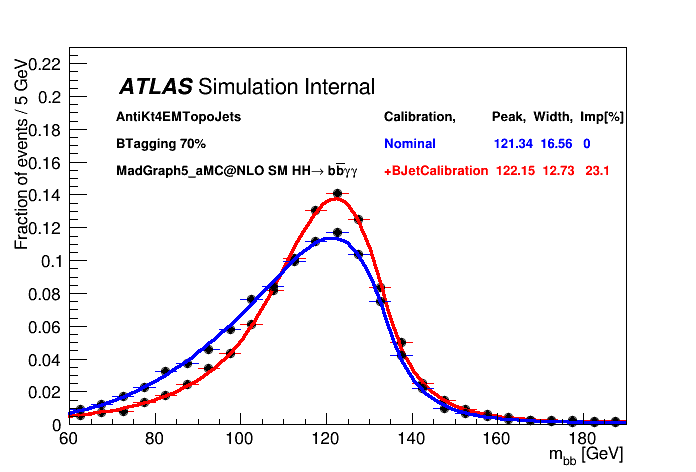
\includegraphics[width=.48\textwidth]{Ch4/Img/mbb_AntiKt4EMTopoJets.png}}\quad
   \subfloat[][]{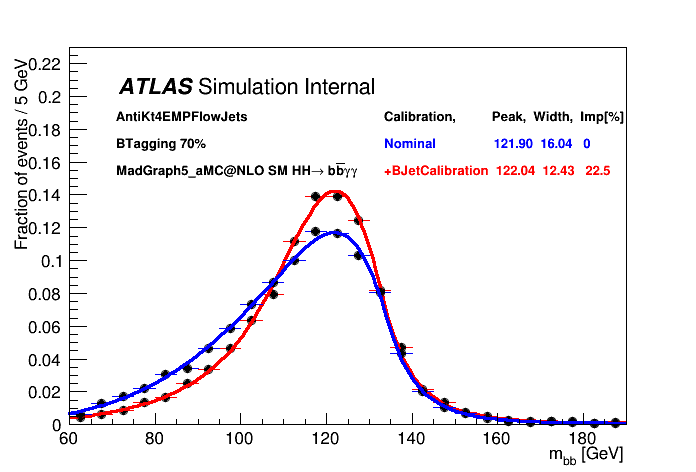
\includegraphics[width=.48\textwidth]{Ch4/Img/mbb_AntiKt4EMPFlowJets.png}}
   \begin{tcolorbox}[colback=black!5!white,colframe=white!75!black]
   \caption{Distribution of $m_{bb}$ before calibration (blue) and after calibration (red) in $HH\rightarrow bb\gamma\gamma$ for (a) topological cluster jets (b) particle flow jets.}
   \label{fig:Jet:Cal:BCal:Result:mbb}
   \end{tcolorbox}
\end{figure}
The two steps $\mu$-in-jet and $p_T$Reco are combined in a decoupled method denoted \bq-jet energy calibration under a simple \texttt{BJetCalibration} tool. The tool is documented and public to be used by analysis with \bq-jet in their final state. It is been the standard \bq-jet calibration across all DiHiggs channels with $b$-jet (\HHyybb, $HH\rightarrow b\bar{b}b\bar{b}$, $HH\rightarrow b\bar{b}\tau\tau$,  $HH\rightarrow b\bar{b}ll+MET$ and $HH\rightarrow b\bar{b}VV$).

\section{Conclusion}
\label{Jet:Conc}
The related features to reconstruct and identify jets and $b$-jets mandatory to reconstruct the \HHyybb events such as reconstruction algorithms, energy calibration, $b$-tagging and the specific $b$-jet calibration are introduced in this chapter. A significant improvement is achieved on the $m_{bb}$ resolution leads to a better signal versus background separation. The developed method shows similar performance to an alternative approach which use a simplified NNs regression to calibrate the \bq-jet energy trained on $t\bar{t}$. The simplified NNs regression uses similar inputs as the decoupled, while the full NNs regression includes additional information about the tracks and secondary vertices ($\sim$90 variables) and achieves a resolution of $\sim$10 GeV in the $m_{bb}$. The huge number of inputs needed by the full NNS regression makes its implementation at the analysis level not trivial and kept for the next analysis round at Run-3.